\documentclass[USenglish]{article}

%\usepackage[utf8]{inputenc}%(only for the pdftex engine)
\RequirePackage[no-math]{fontspec}[2017/03/31]%(only for the luatex or the xetex engine)
\usepackage[small]{dgruyter}

\usepackage{natbib}
\bibliographystyle{apalike}

\usepackage{microtype}

\begin{document}

  \articletype{Research Article}

  \author*[1]{C.J.(Chaojie) Duan}
  %\author[2]{...}
  %\author[1]{...} 
  \runningauthor{Duan}
  \affil[1]{Dulun Consulting Group, research@dulun.com}
  %\affil[2]{...}
  \title{Home Sweet Home Field Advantage:}
  \runningtitle{Bayesian Hierarchical Analysis}
  \subtitle{Examination at Sport, League, and Club Levels}
  \abstract{From 2001 to 2017 seasonal data}
  \keywords{European Professional Soccer Leagues, Home Field Advantage, Poisson generative process}
  %\classification[PACS]{...}
  %\communicated{...}
  %\dedication{...}
  \received{5/21/2018}
  %\accepted{...}
  \journalname{Journal of Quantitative Analysis in Sports}
  %\journalyear{...}
  %\journalvolume{..}
  %\journalissue{..}
  \startpage{1}
  %\aop
  %\DOI{...}
\maketitle

\section{Introduction} 

The popular frequentist (Fisherian) statistical inference process starts with the formulation of an alternative research hypothesis(Ha), such as "people with higher income live happier than low income earners", which is typically set up against a null non-effect hypothesis (Ho), such as ``income level has no effect on happiness". Then researchers collect relevant data (each subject's perceived happiness and income), and conduct a statistical. \citep{Gajewski2006}


\begin{figure}
\caption{Bias - Accuracy Scatter Plot}
{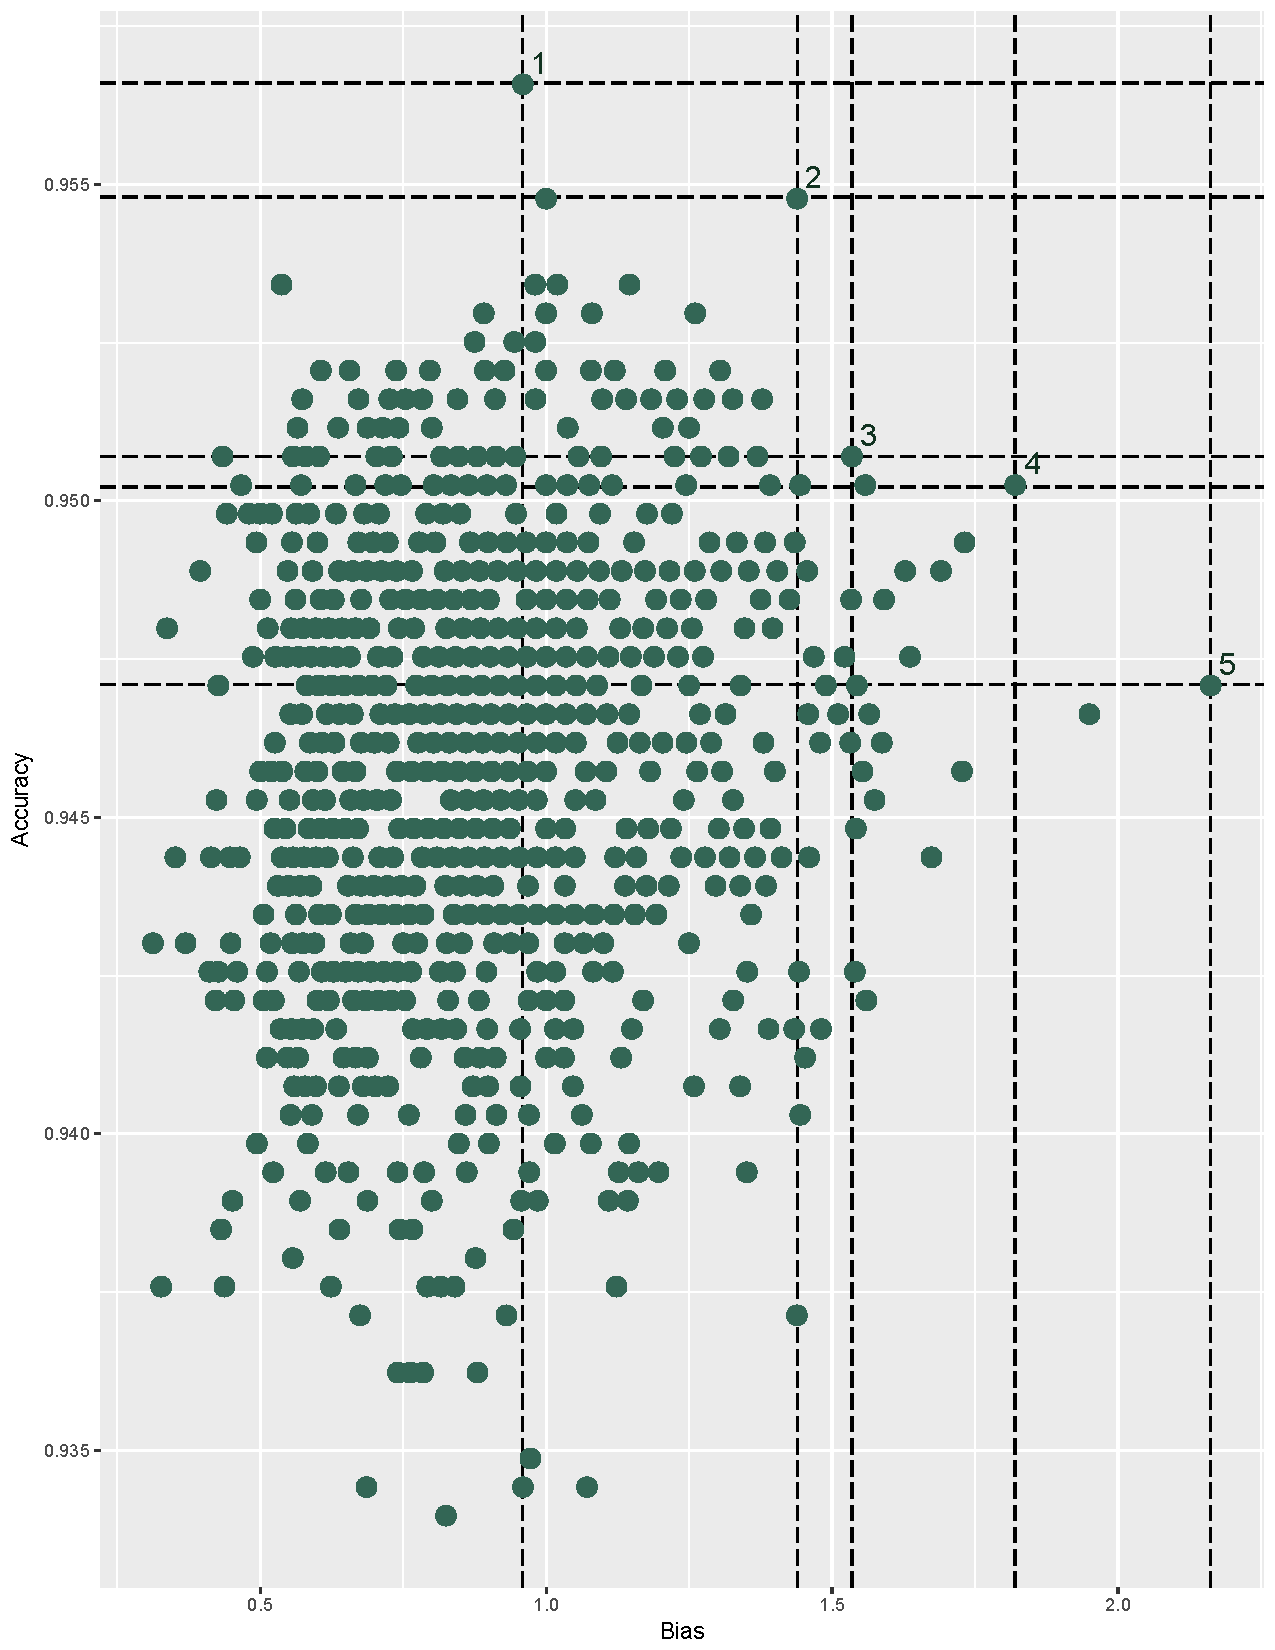
\includegraphics[width=0.65\linewidth]{Rplot04.pdf}}
\label{fig1}
\end{figure}


A second motivator for this study is related to the hotly debated topic of home field advantage in soccer competition.
The contributions we made in this paper are (1) highlighting the different generative process underlying most sports performance metrics and suggesting corresponding solutions.  (2) refuting the long and firmly held belief of HFA: (3) contrasting the Bayesian and the frequentist approaches to statistical inference in answering the the same research question and using the same data.
 
\section{Review of Literature} 

%-----------------------
\begin{table}[ht]
\caption{Descriptive Statistics}
\centering
\begin{tabular}{cccccccc}
\starttabularbody
\hline 
 & Mean & Median & Std. Dev. & Min. & Max. & Skewness & Kurtosis\\
\hline
 MHG & 3.634 & 4 & 1.676 & 0 & 9 & 0.246 & 0.034 \\
\hline 
 MAG & 2.884 & 3 & 1.676 & 0 & 10 & 0.627 & 0.786 \\
\hline
\end{tabular}
\label{tab1}
%{Goal Scoring Metrics: Most Home \& Away Goals at the Season Level} 
\end{table}
%=====================================================

\subsection{Data and Analyses} 

\begin{figure}
\caption{Bias - Accuracy Scatter Plot}
{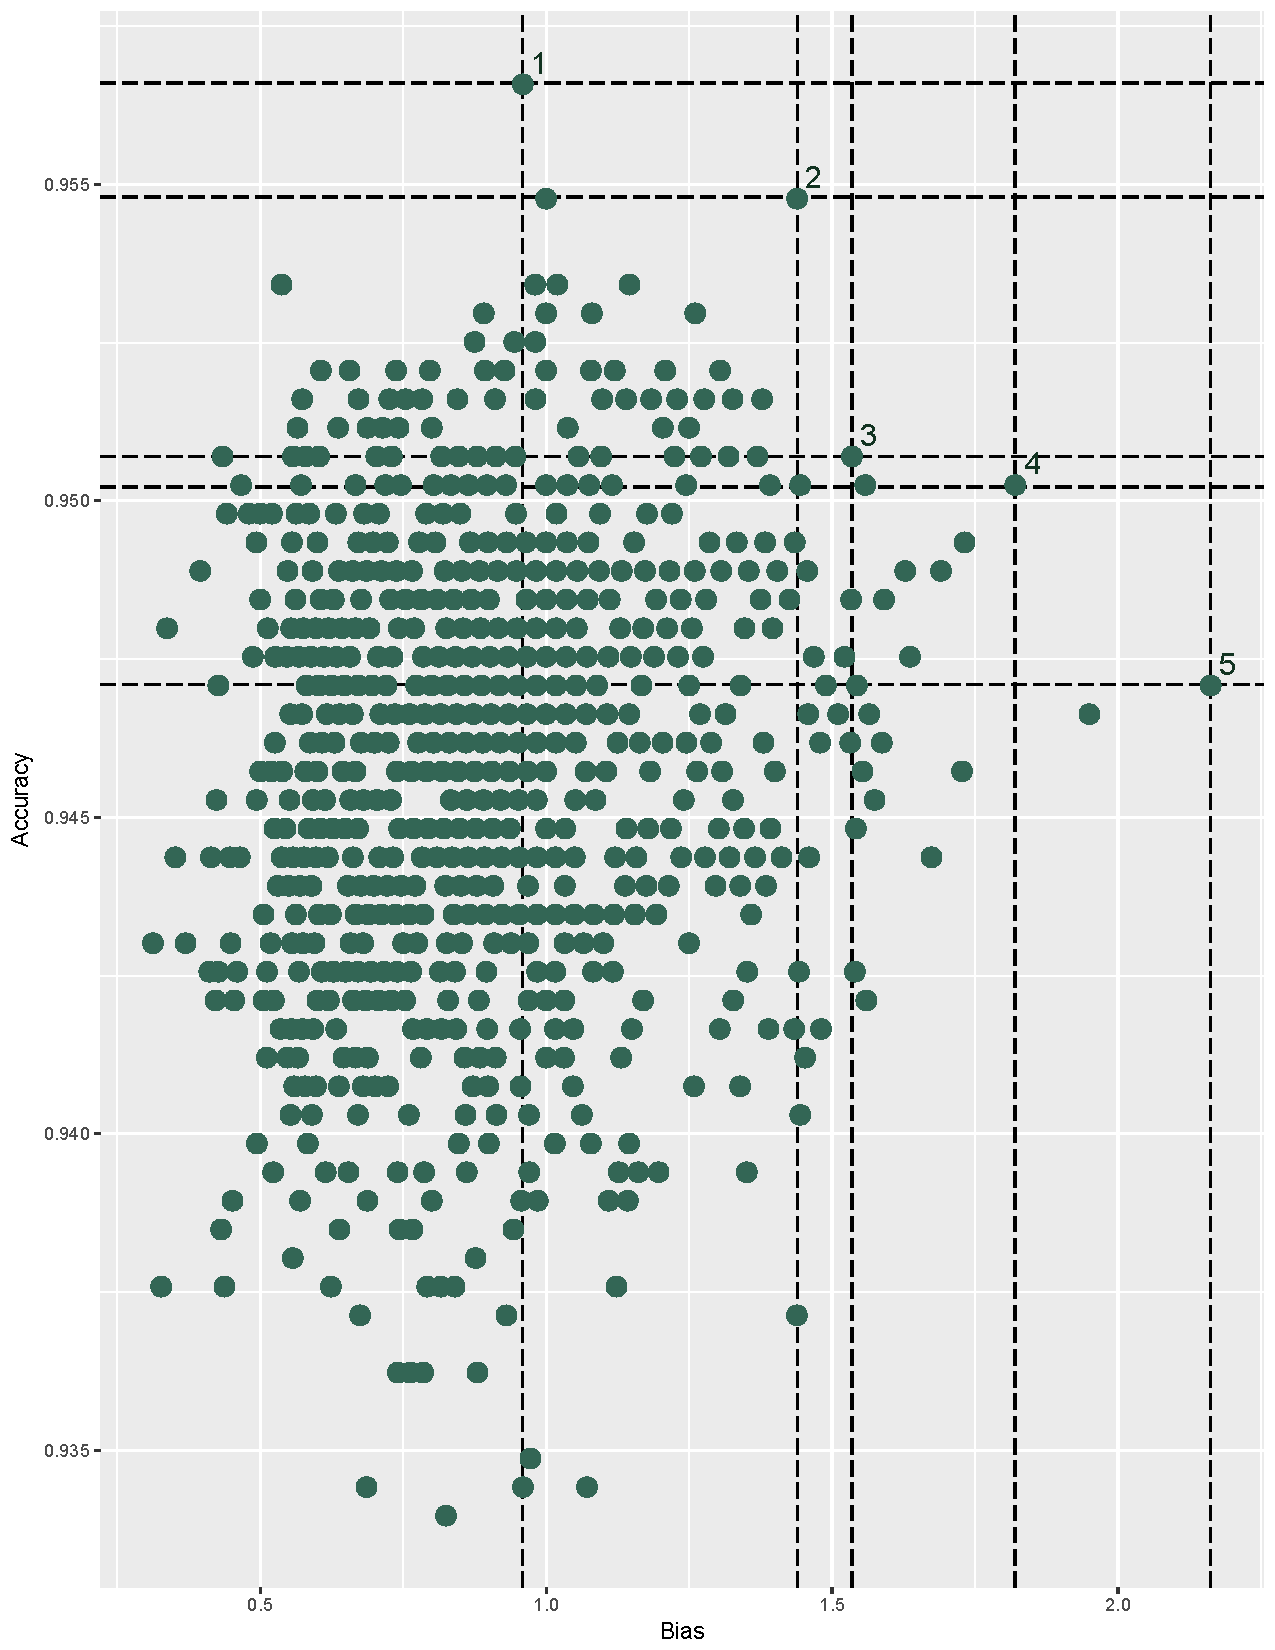
\includegraphics[width=0.65\linewidth]{Rplot04.pdf}}
\label{fig1}
\end{figure}
 

\subsection{Sources} 


 

\begin{acknowledgement}
We would like to thank ESPN FC for compiling the season-level club performance data and allow public access.
\end{acknowledgement}

%\bibliographystyle{name}
\bibliography{Soccer}
\end{document}
